% FIXME1 divide this file into separate ones...
\chapter{Работа с числами с плавающей запятой используя SIMD}

\label{floating_SIMD}
\myindex{IEEE 754}
\myindex{SIMD}
\myindex{SSE}
\myindex{SSE2}
Разумеется, FPU остался в x86-совместимых процессорах в то время, когда ввели расширения \ac{SIMD}.

\ac{SIMD}-расширения (SSE2) позволяют удобнее работать с числами с плавающей запятой.

Формат чисел остается тот же (IEEE 754).

\myindex{x86-64}
Так что современные компиляторы (включая те, что компилируют под x86-64) 
обычно используют \ac{SIMD}-инструкции вместо FPU-инструкций.

Это, можно сказать, хорошая новость, потому что работать с ними легче.

Примеры будем использовать из секции о FPU: \myref{sec:FPU}.

\section{Простой пример}

\lstinputlisting{patterns/12_FPU/1_simple/simple.c}

\subsection{x64}

\lstinputlisting[caption=\Optimizing MSVC 2012 x64]{patterns/205_floating_SIMD/simple_MSVC_2012_x64_Ox.asm}

Собственно, входные значения с плавающей запятой передаются через регистры \XMM{0}-\XMM{3}, 
а остальные --- через стек
\footnote{\href{http://go.yurichev.com/17263}{MSDN: Parameter Passing}}.

$a$ передается через \XMM{0}, $b$\EMDASH{}через \XMM{1}.
Но XMM-регистры (как мы уже знаем из секции о \ac{SIMD}: \myref{SIMD_x86}) 128-битные, 
а значения типа \Tdouble --- 64-битные,
так что используется только младшая половина регистра.

\myindex{x86!\Instructions!DIVSD}
\TT{DIVSD} это SSE-инструкция, означает 
\q{Divide Scalar Double-Precision Floating-Point Values}, 
и просто делит значение типа \Tdouble на другое, лежащие в младших половинах операндов.

Константы закодированы компилятором в формате IEEE 754.

\myindex{x86!\Instructions!MULSD}
\myindex{x86!\Instructions!ADDSD}
\TT{MULSD} и \TT{ADDSD} работают так же, только производят умножение и сложение.

Результат работы функции типа \Tdouble функция оставляет в регистре \XMM{0}.\\
\\
Как работает неоптимизирующий MSVC:

\lstinputlisting[caption=MSVC 2012 x64]{patterns/205_floating_SIMD/simple_MSVC_2012_x64.asm}

\myindex{Shadow space}
Чуть более избыточно. 
Входные аргументы сохраняются в \q{shadow space} (\myref{shadow_space}), 
причем, только младшие половины регистров, т.е. только 64-битные значения типа \Tdouble{}.
Результат работы компилятора GCC точно такой же.

\subsection{x86}

Скомпилируем этот пример также и под x86. MSVC 2012 даже генерируя под x86, использует SSE2-инструкции:

\lstinputlisting[caption=\NonOptimizing MSVC 2012 x86]{patterns/205_floating_SIMD/simple_MSVC_2012_x86.asm}

\lstinputlisting[caption=\Optimizing MSVC 2012 x86]{patterns/205_floating_SIMD/simple_MSVC_2012_x86_Ox.asm}

Код почти такой же, правда есть пара отличий связанных с соглашениями о вызовах:

1) аргументы передаются не в XMM-регистрах, а через стек, как и прежде, в примерах с FPU (\myref{sec:FPU});

2) результат работы функции возвращается через \ST{0} --- для этого он через стек
(через локальную переменную \TT{tv}) копируется из XMM-регистра в \ST{0}.

\clearpage
Попробуем соптимизированный пример в \olly:

\begin{figure}[H]
\centering
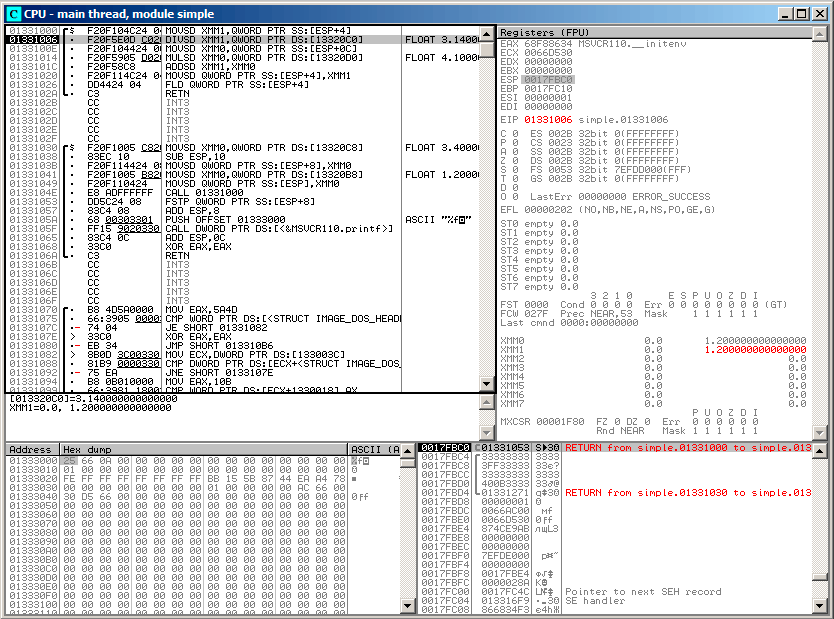
\includegraphics[scale=\FigScale]{patterns/205_floating_SIMD/simple_olly1.png}
\caption{\olly: \TT{MOVSD} загрузила значение $a$ в \XMM{1}}
\label{fig:FPU_SIMD_simple_olly1}
\end{figure}

\clearpage
\begin{figure}[H]
\centering
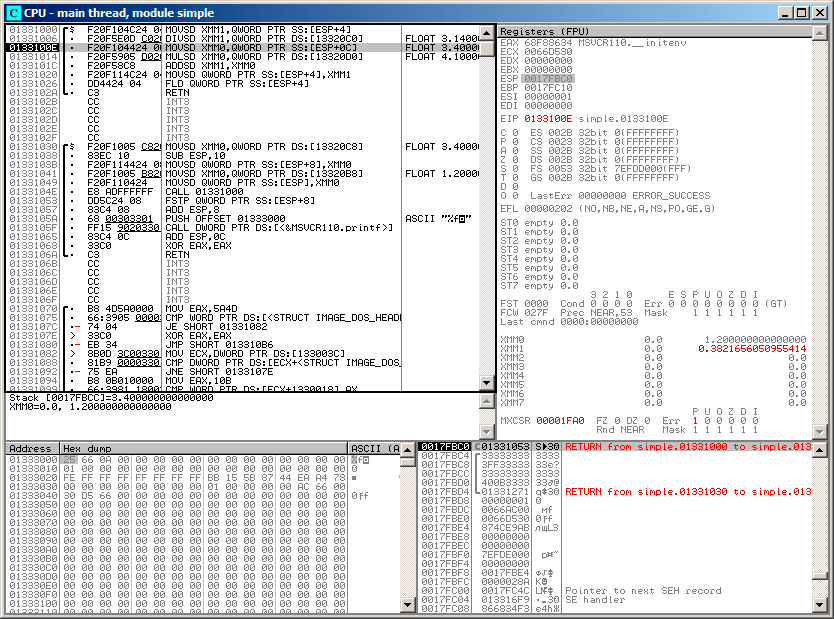
\includegraphics[scale=\FigScale]{patterns/205_floating_SIMD/simple_olly2.png}
\caption{\olly: \TT{DIVSD} вычислила \gls{quotient} 
и оставила его в \XMM{1}}
\label{fig:FPU_SIMD_simple_olly2}
\end{figure}

\clearpage
\begin{figure}[H]
\centering
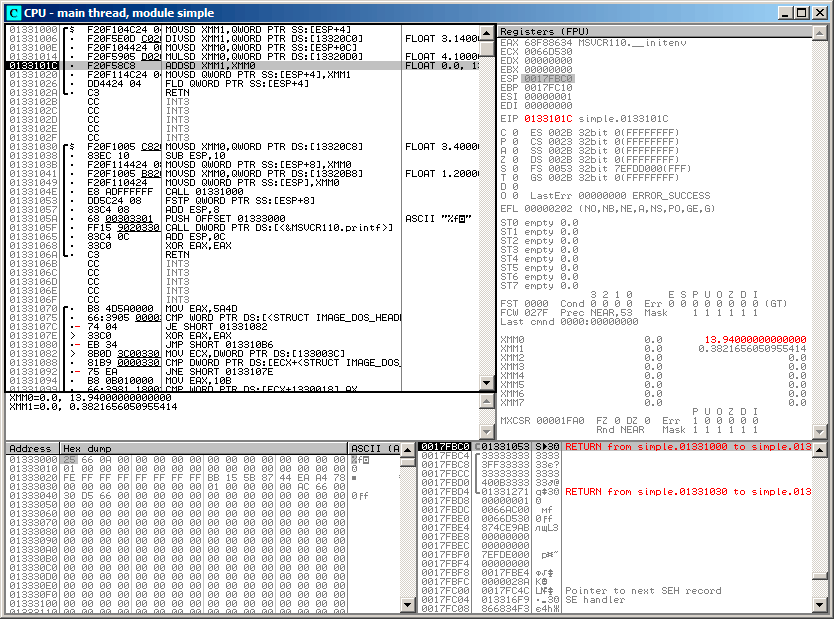
\includegraphics[scale=\FigScale]{patterns/205_floating_SIMD/simple_olly3.png}
\caption{\olly: \TT{MULSD} вычислила \gls{product} и оставила его в \XMM{0}}
\label{fig:FPU_SIMD_simple_olly3}
\end{figure}

\clearpage
\begin{figure}[H]
\centering
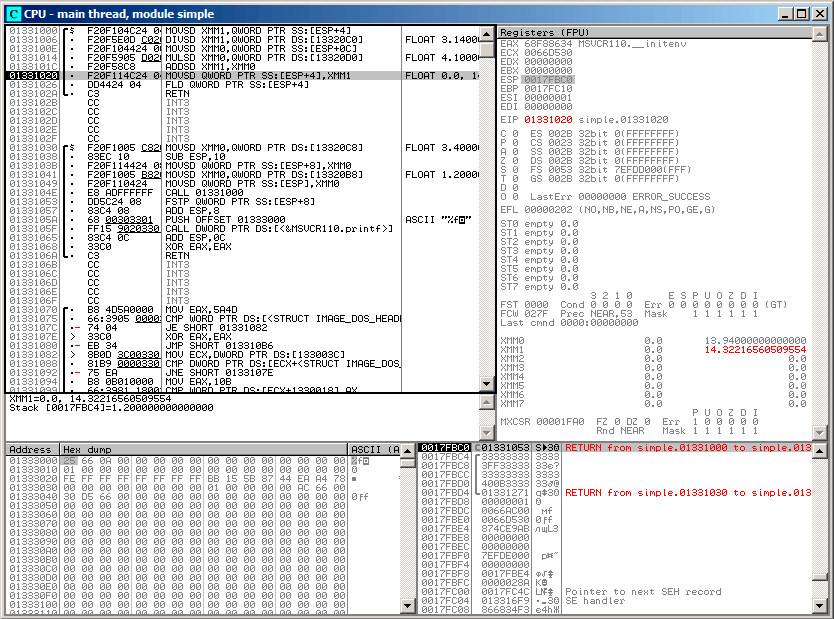
\includegraphics[scale=\FigScale]{patterns/205_floating_SIMD/simple_olly4.png}
\caption{\olly: \TT{ADDSD} прибавила значение в \XMM{0} к \XMM{1}}
\label{fig:FPU_SIMD_simple_olly4}
\end{figure}

\clearpage
\begin{figure}[H]
\centering
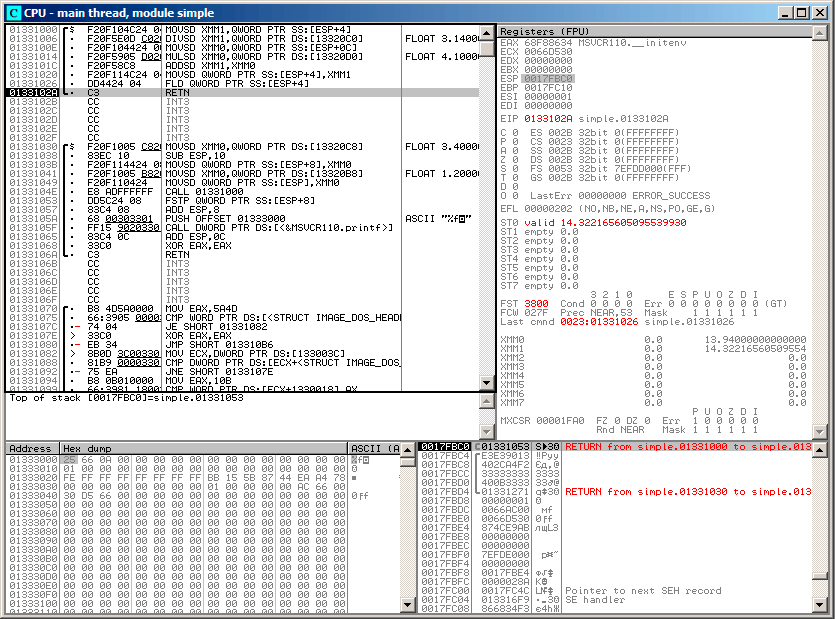
\includegraphics[scale=\FigScale]{patterns/205_floating_SIMD/simple_olly5.png}
\caption{\olly: \FLD оставляет результат функции в \ST{0}}
\label{fig:FPU_SIMD_simple_olly5}
\end{figure}

Видно, что \olly показывает XMM-регистры как пары чисел в формате \Tdouble,
но используется только \IT{младшая} часть.

Должно быть, \olly показывает их именно так, потому что сейчас исполняются SSE2-инструкции
с суффиксом \TT{-SD}.

Но конечно же, можно переключить отображение значений в регистрах и посмотреть содержимое
как 4 \Tfloat{}-числа или просто как 16 байт.

\clearpage
\section{Передача чисел с плавающей запятой в аргументах}

\lstinputlisting{patterns/12_FPU/2_passing_floats/pow.c}

Они передаются в младших половинах регистров \XMM{0}-\XMM{3}.

\lstinputlisting[caption=\Optimizing MSVC 2012 x64]{patterns/205_floating_SIMD/pow_MSVC_2012_x64_Ox.asm}

\myindex{x86!\Instructions!MOVSD}
\myindex{x86!\Instructions!MOVSDX}
Инструкции \TT{MOVSDX} нет в документации от Intel и AMD  (\myref{x86_manuals}), там она называется просто \TT{MOVSD}.
Таким образом, в процессорах x86 две инструкции с одинаковым именем (о второй: \myref{REP_MOVSx}).
Возможно, в Microsoft решили избежать путаницы и переименовали инструкцию в \TT{MOVSDX}.
Она просто загружает значение в младшую половину XMM-регистра.

Функция \TT{pow()} берет аргументы из \XMM{0} и \XMM{1}, 
и возвращает результат в \XMM{0}.
Далее он перекладывается в \RDX для \printf. 
Почему? 
Может быть, это потому что 
\printf --- функция с переменным количеством аргументов?

\lstinputlisting[caption=\Optimizing GCC 4.4.6 x64]{patterns/205_floating_SIMD/pow_GCC446_x64_O3_RU.s}

GCC работает понятнее. 
Значение для \printf передается в \XMM{0}. 
Кстати, вот тот случай, когда в \EAX
для \printf записывается 1 --- это значит, что будет передан один аргумент в векторных регистрах, 
так того требует стандарт \SysVABI.

\section{Пример с сравнением}

\lstinputlisting{patterns/12_FPU/3_comparison/d_max.c}

\subsection{x64}

\lstinputlisting[caption=\Optimizing MSVC 2012 x64]{patterns/205_floating_SIMD/d_max_MSVC_2012_x64_Ox.asm}

\Optimizing MSVC генерирует очень понятный код.

\myindex{x86!\Instructions!COMISD}
Инструкция \TT{COMISD} это \q{Compare Scalar Ordered Double-Precision Floating-Point 
Values and Set EFLAGS}. Собственно, это она и делает.\\
\\
\NonOptimizing MSVC генерирует более избыточно, но тоже всё понятно:

\lstinputlisting[caption=MSVC 2012 x64]{patterns/205_floating_SIMD/d_max_MSVC_2012_x64.asm}

\myindex{x86!\Instructions!MAXSD}
А вот GCC 4.4.6 дошел в оптимизации дальше и применил инструкцию \TT{MAXSD} (\q{Return Maximum Scalar 
Double-Precision Floating-Point Value}), которая просто выбирает максимальное значение!

\lstinputlisting[caption=\Optimizing GCC 4.4.6 x64]{patterns/205_floating_SIMD/d_max_GCC446_x64_O3.s}

\clearpage
\subsection{x86}

Скомпилируем этот пример в MSVC 2012 с включенной оптимизацией:

\lstinputlisting[caption=\Optimizing MSVC 2012 x86]{patterns/205_floating_SIMD/d_max_MSVC_2012_x86_Ox.asm}

Всё то же самое, только значения $a$ и $b$ 
берутся из стека, а результат функции оставляется в \ST{0}.

Если загрузить этот пример в \olly, 
увидим, как инструкция \TT{COMISD} сравнивает значения и устанавливает/сбрасывает
флаги \CF и \PF:

\begin{figure}[H]
\centering
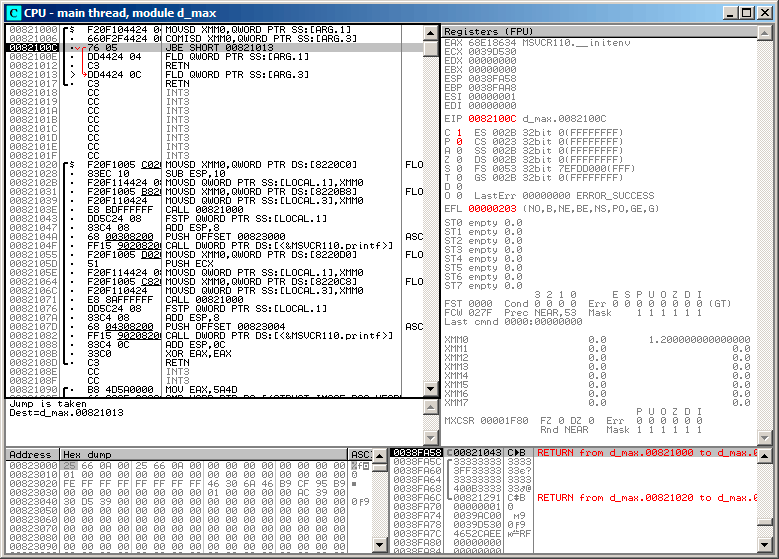
\includegraphics[scale=\FigScale]{patterns/205_floating_SIMD/d_max_olly.png}
\caption{\olly: \TT{COMISD} изменила флаги \CF и \PF}
\label{fig:FPU_SIMD_d_max_olly}
\end{figure}

\section{Вычисление машинного эпсилона: x64 и SIMD}
\label{machine_epsilon_x64_and_SIMD}

Вернемся к примеру \q{вычисление машинного эпсилона} для \Tdouble \lstref{machine_epsilon_double_c}.

Теперь скомпилируем его для x64:

\lstinputlisting[caption=\Optimizing MSVC 2012 x64]{patterns/205_floating_SIMD/epsilon_double_MSVC_2012_x64_Ox.asm}

Нет способа прибавить 1 к значению в 128-битном XMM-регистре, так что его нужно в начале поместить в память.

Впрочем, есть инструкция ADDSD (\IT{Add Scalar Double-Precision Floating-Point Values}),
которая может прибавить значение к младшей 64-битной части XMM-регистра игнорируя старшую половину,
но наверное MSVC 2012 пока недостаточно хорош для этого

\footnote{В качестве упражнения, вы можете попробовать переработать этот код, чтобы избавиться 
от использования локального стека.}.

Так или иначе, значение затем перезагружается в XMM-регистр и происходит вычитание.

SUBSD это \q{Subtract Scalar Double-Precision Floating-Point Values}, 
т.е. операция производится над младшей 64-битной частью 128-битного XMM-регистра.
Результат возвращается в регистре XMM0.

\sectionold{И снова пример генератора случайных чисел}
\label{FPU_PRNG_SIMD}

Вернемся к примеру \q{пример генератора случайных чисел} \lstref{FPU_PRNG}.

Если скомпилировать это в MSVC 2012, компилятор будет использовать SIMD-инструкции для FPU.

\lstinputlisting[caption=\Optimizing MSVC 2012]{patterns/205_floating_SIMD/FPU_PRNG/MSVC2012_Ox_Ob0_RU.asm}

% FIXME1 rewrite!
У всех инструкций суффикс -SS, это означает \q{Scalar Single}.

\q{Scalar} означает что только одно значение хранится в регистре.

\q{Single} означает что это тип \Tfloat.



\section{Итог}

Во всех приведенных примерах, в XMM-регистрах используется только младшая половина регистра, там
хранится значение в формате IEEE 754.

Собственно, все инструкции с суффиксом 
\TT{-SD} (\q{Scalar Double-Precision}) --- это инструкции для работы с числами с плавающей 
запятой в формате IEEE 754, 
хранящиеся в младшей 64-битной половине XMM-регистра.

Всё удобнее чем это было в FPU, видимо, сказывается тот факт, что расширения 
SIMD развивались не так хаотично как FPU в прошлом.

Стековая модель регистров не используется.

\myindex{x86!\Instructions!ADDSS}
\myindex{x86!\Instructions!MOVSS}
\myindex{x86!\Instructions!COMISS}
% TODO1: do this!
Если вы попробуете заменить в этих примерах \Tdouble на \Tfloat{}, то инструкции будут использоваться те же,
только с суффиксом
% FIXME1 ... but their -SS versions
 \TT{-SS} 
(\q{Scalar Single-Precision}), например, \TT{MOVSS}, \TT{COMISS}, \TT{ADDSS}, итд.

\q{Scalar} означает что SIMD-регистр будет хранить только одно значение, вместо нескольких.

Инструкции, работающие с несколькими значениями в регистре одновременно, имеют \q{Packed} в названии.

Нужно также обратить внимание, что SSE2-инструкции работают с 64-битными числами (\Tdouble) в формате IEEE 754,
в то время как внутреннее представление в FPU --- 80-битные числа.

Поэтому ошибок округления (\IT{round-off error}) в FPU может быть меньше чем в SSE2,
как следствие, можно сказать, работа с FPU может давать более точные результаты вычислений.

